\chapter{TESTES} % (fold)
\label{cha:testes} % (fold)

\section{Descrição do Experimento}
\label{cha:descricao_do_experimento}

 Inicialmente 12 pessoas serão convidadas a participar do experimento. Cada uma das 12 pessoas deverá convidar outras 4 pessoas para formarem um grupo de amigos. Sendo assim, formam-se 12 grupos de 5 amigos, totalizando 60 pessoas. Cada pessoa que participar de um grupo de amigos deverá concordar em ser definida como amiga de todos no grupo, ou seja, todas as pessoas pertencentes a um mesmo grupo de amigos se conhecem e se consideram amigas.

 Cada uma das 12 pessoas receberá 5 Termos de Consentimento Livre e Esclarecido (TCLE) para que seja lido e assinado por todos que concordaram em participar do grupo e, sendo assim, do experimento. Após ler e assinar o TCLE a pessoa torna-se um participante do experimento e deve informar o seu e-mail para a pessoa que lhe convidou. De posse dos e-mails de todos presentes no grupo de amigos, cada uma das 12 pessoas deverá enviá-los aos pesquisadores.

 Um e-mail será enviado a cada um dos 60 participantes com um endereço da internet para que ele possa se cadastrar no sistema do experimento. Os grupos de amigos já serão formados no sistema com base nos endereços de e-mail enviados por cada uma das 12 pessoas que foram incialmente convidadas a participar. Os participantes deverão informar os seguintes dados no cadastro:

\begin{itemize}
	\item Nome
	\item Sexo
	\item Faixa etária (18-25, 26-30, 30-40, +40)
	\item Foto (Não obrigatório. Caso queira, o participante poderá escolher uma foto sua para representar o seu perfil no sistema.)
\end{itemize}

 Após isso, o participante deverá escolher a opção de salvar os seus dados e então será remetido a outra página do sistema que mostrará uma lista com 20 produtos escolhidos pelos pesquisadores. Tais produtos serão escolhidos com base na sua popularidade definida no site www.submarino.com. O participante deverá avaliar TODOS os 20 produtos para passar para a próxima fase do experimento.

 Avaliar um produto significa dizer o quanto o participante acha aquele produto relevante para si, ou seja, o quanto ele gosta do produto. A avaliação é feita por meio da atribuição de uma nota de 1 a 5, sendo 1 o produto ser irrelevante ou inútil ao participante e 5 o produto ser completamente relevante ou muito útil a ele. 

 Caso o participante não conheça o produto, ou seja, não tivesse ouvido falar daquele produto ou não tivesse conhecimento suficiente para reconhecê-lo, até o instante em que o produto lhe foi apresentado pelo sistema, ele deve escolher a opção "Não conheço", Neste caso a opção de avaliar o produto será desabilitada, pois não é de interesse do sistema saber da opinião do participante sobre um produto que ele não tem conhecimento algum.

 Selecionando a opção "Não conheço", o sistema não atribuirá nota à avaliação do produto na base de dados do participante, marcando apenas com uma flag booleana indicando que o participante não conhece o produto. Um produto que não é conhecido pelo usuário, e sendo assim não avaliado pelo mesmo, não deverá ser utilizado no algoritmo de recomendação, porém a informação de não conhecimento por parte do usuário deverá ser guardada na base de dados para posterior análise. Além disso, o participante poderá avaliar o produto posteriormente, caso tenha procurado saber a respeito do mesmo.

 Terminadas as avaliações dos 20 produtos, o participante verá uma listagem aleatória dos produtos cadastrados no sistema. Ele deverá procurar e avaliar - a avaliação deve ser feita da mesma forma como anteriormente - 10 produtos de sua escolha. Neste caso, o participante deverá avaliar apenas produtos de seu conhecimento, sendo que a opção de "Não conheço" não estará disponível.

 Os produtos poderão ser localizados a partir da filtragem de categorias e de um campo de busca por texto, onde o participante digita o nome do produto e o sistema o procura na base de dados, atualizando a lista com os resultados obtidos. As categorias de produtos presentes no sistema são:

\begin{itemize}
	\item Roupas
	\item Músicas
	\item Filmes
	\item Eletrônicos
	\item Livros
\end{itemize}

 Para facilidade do participante, o sistema exibirá na tela o número de produtos restantes a serem avaliados.

 O sistema aguardará todos os participantes avaliarem os 20 produtos escolhidos pelos pesquisadores e os 10 produtos escolhidos por eles. Somente quando todos terminarem as etapas de avaliação de produtos que a etapa seguinte estará disponível. Esse sincronismo é necessário porque o sistema precisa que todas as informações de todos os participantes estejam disponíveis na base de dados. Neste meio tempo, o participante que já finalizou as suas tarefas receberá uma mensagem do sistema indicando que ele receberá um e-mail quando a próxima etapa estiver liberada.
 
 Assim que os todos os produtos forem avaliados, o sistema mostrará as fotos com o nome dos 4 amigos do grupo do participante e uma área com listagem aleatória de produtos cadastrados no sistema. Será solicitado ao participante que ele realize 5 recomendações a cada um dos quatro amigos do seu grupo, totalizando assim 20 recomendações a serem feitas. Para isso, o participante localiza um produto no sistema e escolhe a opção de recomendar a uma pessoa. Desse modo, será exibida a tela de recomendação de produto, com as informações do produto escolhido e uma lista com seus quatro amigos. O participante escolhe para quais amigos ele recomendará aquele produto e confirma a recomendação.
 
 O propósito das recomendações é que apenas boas recomendações sejam realizadas pelos participantes. Uma boa recomendação é a indicação de um produto que o participante acha que seu amigo gostará e será relevante a ele naquele momento.

 Depois de fazer as 5 recomendações a cada amigo do seu grupo, o sistema mostrará ao participante uma lista contendo foto e nome de 10 participantes que não façam parte do seu grupo e solicitará a ele que recomende apenas 1 produto a cada uma dessas pessoas, totalizando 10 recomendações. Para poder fazer boas recomendações, o participante terá acesso às avaliações de produtos feitas por estas pessoas, além das informações de cadastro de cada uma delas. Para facilitar tal tarefa, o sistema indicará ao participantes quais das 10 pessoas ainda não receberam a sua recomendação.

 O sistema aguardará todos os participantes finalizarem as etapas de recomendar produtos aos amigos e aos desconhecidos antes de continuar o experimento. Neste meio tempo, o participante que já finalizou as suas tarefas receberá uma mensagem do sistema indicando que ele receberá um e-mail quando a próxima etapa estiver liberada. Após a conclusão das etapas de recomendação por parte de todos os participantes, será enviado um e-mail a cada participante solicitando a continuação do experimento.
 
 Ao entrar novamente no sistema o participante visualizará 20 recomendações de produtos. Estas são compostas de 5 recomendações feitas pelos seus amigos, 5 recomendações feitas por desconhecidos - em ambos os casos escolhidas aleatoriamente pelo sistema - e 10 recomendações feitas pelo sistema utilizando os algoritmos de recomendação com base em similaridade entre perfis e entre produtos. Nesta etapa, chamada de "teste cego", não ficará visível ao participante quem é o autor da recomendação. Isso é feito para que não haja nenhuma influência sobre ele quando for avaliar a recomendação.
 
 A avaliação da recomendação consiste no participante dizer se gostou ou não da recomendação daquele produto a ele e se ela o surpreendeu positivamente. O participante também deverá avaliar o produto, da mesma maneira que avaliou produtos anteriormente. O sistema mostrará quantas recomendações restam para serem avaliadas pelo participante.
 
 Após avaliar as 20 recomendações, o participante receberá outras 30 recomendações. Neste caso serão utilizadas as 15 recomendações restantes realizadas pelos seua amigos, as 5 recomendações restantes feitas a ele por desconhecidos e 10 recomendações feitas pelo sistema utilizando o algoritmo de recomendação com base na confiança. Nesta etapa ficará visível ao participante quem é o autor da recomendação (inclusive quando for o sistema). Após terminar de avaliar todas as recomendações, o experimento será finalizado e uma mensagem de agradecimento será mostrada ao participante.
 
 \section{Protótipo}
 \label{cha:prototipo}

 Um protótipo do sistema foi desenvolvido para que se pudesse ter noção da usabilidade e do funcionamento do sistema de recomendação. Inicialmente as recomendações são realizadas sem levar em conta os dados de confiança e reputação entre usuários. A Figura~\ref{fig:tela_inicial_prototipo} mostra a página inicial do protótipo, contendo a listagem dos primeiros produtos presentes na base de dados e a opção do usuário fazer o \textit{login} no sistema.
 
\begin{figure}
  \centering
  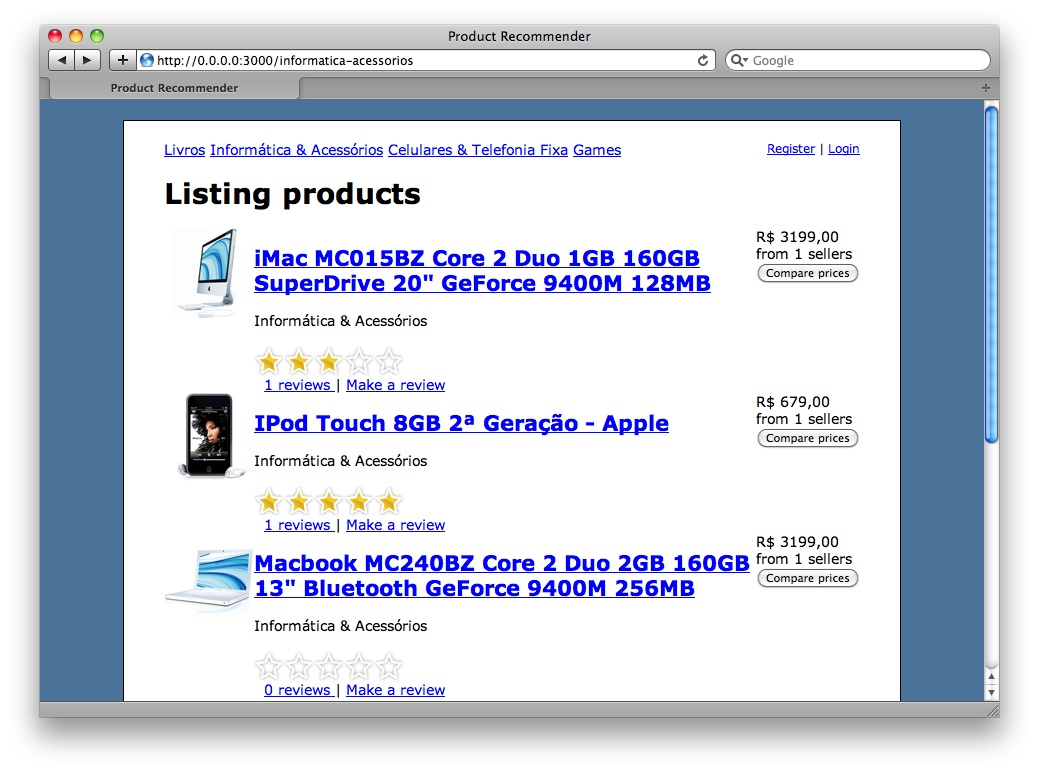
\includegraphics[width=\textwidth]{imagens/Tela_Inicial_Prototipo}
  \caption{\it Tela inicial do protótipo}
  \label{fig:tela_inicial_prototipo}
\end{figure}

 Para se cadastrar, a pessoa necessita apenas informar o seu nome de usuário, e-mail e entrar com uma senha pessoal. A tela de \textit{login} solicita apenas o nome de usuário e senha. Após a validação dos dados, o sistema retorna para a tela inicial para que o usuário possa detalhar um produto de seu interesse. Há a opção de avaliar o produto sem conferir os seus detalhes. Para avaliar o produto o usuário escolhe de 1 a 5, sendo 1 não gostar do produto e 5 gostar muito, e clicar em uma das cinco estrelas. O número de estrelas coloridas mostra a nota da avaliação. 
 
 Para efetuar o \emph{login} o sistema solicita apenas o nome de usuário e senha. Após a autenticação, o sistema retorna para a tela inicial para que o usuário possa procurar um produto de seu interesse. Ao escolher um produto, o sistema abre os seus detalhes incluindo nome, foto e descrição completa, como mostra a Figura~\ref{fig:detalhe_produto_prototipo}.

\begin{figure}
  \centering
  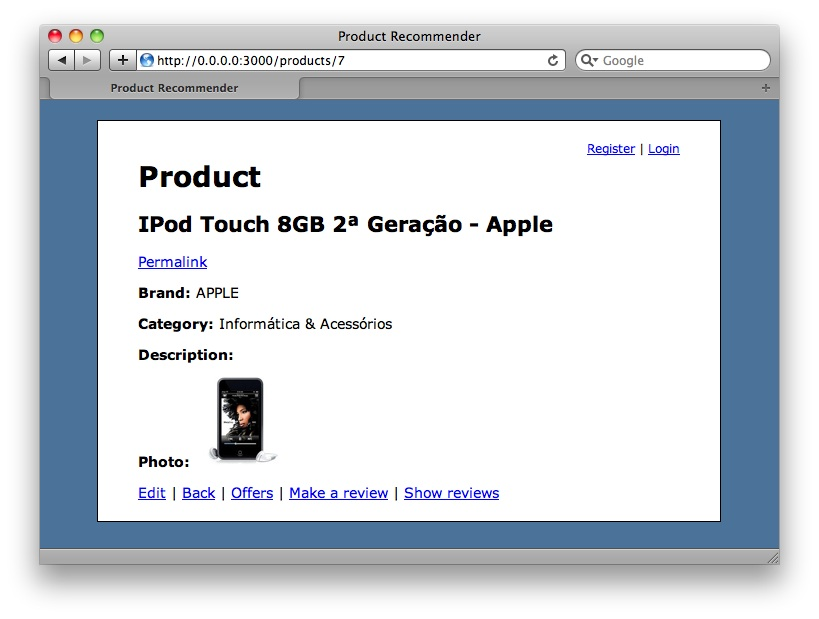
\includegraphics[width=\textwidth]{imagens/Detalhe_Produto_Prototipo}
  \caption{\it Detalhe do produto}
  \label{fig:detalhe_produto_prototipo}
\end{figure}

 Na tela de detalhamento do produto o usuário poderá editar as informações do mesmo ao escolher a opção \textit{edit}. Também é possível visualizar os comentários (\textit{reviews}) feitos pelos usuários sobre o produto detalhado, além de fazer o seu próprio comentário, clicando em \textit{Make a review}.
  
 A encontrar um produto interessante o usuário tem a opção de recomendá-lo para outros da rede social. A opção \emph{Recommend it!} leva o usuário a tela ilustrada na Figura~\ref{fig:recomendacao_produto_prototipo}, onde é possível selecionar os amigos para os quais a recomendação será enviada.         
 
 \begin{figure}
   \centering
   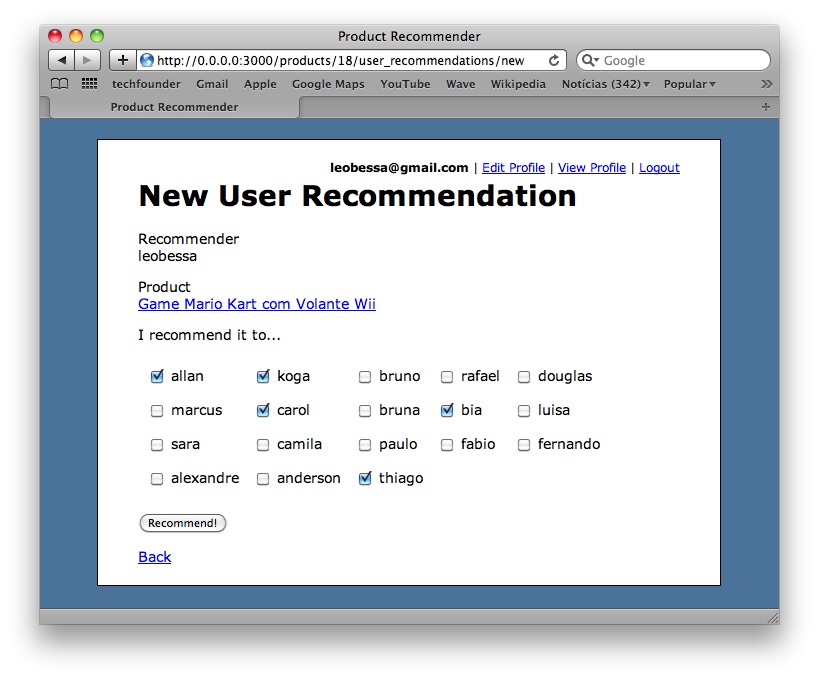
\includegraphics[width=\textwidth]{imagens/TELA_RECOMENDACAO_PROTOTIPO}
   \caption{\it Tela de recomendação de produto}
   \label{fig:recomendacao_produto_prototipo}
 \end{figure}
